\documentclass[14pt,fleqn]{article}
\usepackage{graphicx}
\usepackage[T1]{fontenc}
\usepackage[utf8]{inputenc}
\usepackage[french]{babel}
\usepackage{amsmath}
\usepackage{amssymb}
\usepackage{amscd}
\usepackage{latexsym}
\usepackage{tabularx}
\usepackage{a4wide}
%\usepackage{here}
\usepackage{enumerate}
%\usepackage{subfigure}
%\usepackage{stmaryrd}
%\usepackage{vmargin}
\usepackage{url}
\usepackage{marvosym} % Pour les euros

\usepackage{float}
\usepackage{subfig}
%\usepackage[textwidth=16cm,textheight=23cm,includefoot]{geometry}


%\renewcommand{\baselinestretch}{1.05}\small\normalsize


\newtheorem{theorem}{Theorem}
\newtheorem{conjecture}[theorem]{Conjecture}
\newtheorem{question}{Question}


\begin{document}

 \begin{figure}[H]
  \centering
  \subfloat  
{
\includegraphics[scale=1]{iflogo-azur-sable-150x60_0.png}  
}
 \hfill
  \subfloat
  {
\includegraphics[scale=.4]{gscop.png}  
}

\end{figure}


\begin{center}
\line(1,0){450}

\vspace{0.2in}
{\huge \bf ToFu: Topologie eFfective et calcUl}
\vspace{0.2in}
\line(1,0){450}
\bigskip

Projet équipe-action  \\
Mathematics: from Fundamentals to Applications
\\
Porteurs du projet:  {\bf Greg McShane} (IF),  {\bf Francis Lazarus} (G-SCOP)
\end{center}


\tableofcontents

\newpage

\section{Presentation of the team}
The team consists of eight members in total (7 tenured faculty and one PhD student : Joanny Perret) du projet belonging to two  laboraties on the Grenoble campus : \\
Institut Fourier (IF) and G-SCOP.

\smallskip
\vspace{.5cm}
\begin{center}
\begin{tabular}[h]{|c|c|c|l|l|}
  \hline
 Laboratoire & Équipe & Nom \\
\hline \hline
IF & Géométrie et Topologie & {\bf Martin Deraux} &\\
\hline
G-SCOP & Optimisation Combinatoire & {\bf Louis Esperet}& \\
\hline
G-SCOP & Optimisation Combinatoire & {\bf Francis Lazarus}& 
francis.lazarus@gipsa-lab.grenoble-inp.fr\\
\hline
IF & Géométrie et Topologie & {\bf Greg McShane}&
mcshane@univ-grenoble.fr \\
\hline
IF & Géométrie et Topologie & {\bf Anne Parreau}& \\
\hline
G-SCOP & Optimisation Combinatoire & {\bf Joanny Perret}& \\
\hline
IF & Géométrie et Topologie & {\bf Andrea Seppi}& \\
\hline
G-SCOP & Optimisation Combinatoire & {\bf Mat\v{e}j Stehlìk}& \\
\hline
\end{tabular}
\end{center}

\section{Synopsis}
%\textbf{
%    le sujet et son contexte,\\
%    les défis scientifiques ciblés\\
%   leur positionnement par rapport aux thématiques du labex
%}


The purpose of the present project is to develop a synergy between colleagues with a backgrounds in fundamental mathematics  and others coming from more an applied/computer science background in order to study important problems related to the complexity of topological spaces 
(such as surfaces but more generally manifolds with particular geometric structures) 
and initiate investigations using computer software.
The problems we intend to study
are those which have both 
combinatorial and analytical aspects. Past experience shows that
this kind of problem 
has often lead to rich exchanges between 
those  
who have a purely theoretical background 
on one side 
and a more  applied/numerical one
on the other.

We believe that by combining the knowledge of theoretical
mathematicians and computer scientists
present on the Grenoble campus 
we can make significant progress 
on a number of geometric problems 
which have an analytic, combinatorial and algorithmic nature. 
This is something we have come to realise collectively
in the past few years 
through participating together in seminars at IF and G-SCOP, in evaluation committees for our PhD students 
and in workshops.


\section{Research Context}

In this project we aim to study ways to describe the geometry of space from two points of view: 
\begin{itemize}
\item combinatorial/analytic
\item analytical
\end{itemize} 
This double headed approach has been central to the field of low dimensional topology since its inception.
It  has proven spectacularly successful 
particularly now that computers allow us 
to make very accurate calculations rapidly as we shall now see. 



\subsection{Thurston and SnapPea}

The dual analytic/combinatorial approach was pioneered by the likes of Felix Klein, Henri Poincaré and Max Dehn in the late 19th century and early 20th century.
They studied surfaces
 and 3  manifolds using  
differential equations,
combinatorial constructions
and transformation groups.
Of particular note was the proof of  the classification of triangulated surfaces in 1907 by Dehn which uses a clever algorithm. 
Nearly 100 years later Bill Thurston
used complex analytic techniques to prove
existence theorems 
for hyperbolic structures on 3 manifolds
\cite{Thu1}
-- that is to show that the fundamental group of the 3 manifold is isomorphic
to a discrete group of isometries of 
hyperbolic 3 space.
Thurston's results are 
is based on fixed point 
theorems on \textit{Teichmuller space}
and are non constructive.
Though very elegant 
they were certainly not \textit{effective}.
With the advent of computers 
there were many new possibilities
for constructing and exploring Thurston's manifolds.
Jeffrey Weeks,  as part of his 1985 doctoral thesis
supervised by Thurston,
created a remarkable piece of software called SnapPea which tries to find a
hyperbolic structure on the complement of a knot.
To do this it starts  by finding a good  decomposition of the  space into tetrahedra analogous in some sense 
to Dehn's triangulation of a surface.
It then associates to each tetrahedron a complex number 
and constructs a
set of nonlinear equations of complex variables from the adjacencies between the tetrahedra.
A solution of this system  gives a complete hyperbolic metric on the space.
SnapPea  uses an iterative method -  essentially Newton's method - to search for solutions. 
Once a solution is found many 
invariants of the manifold can be computed: volume, Chern-Simons invariant, etc.
One can also understand relations to other 3-manifolds which are related to it 
 by doing \textit{Dehn surgery}.
 
SnapPea has proven to be a very useful piece of software. It has been used to verify conjectures in base cases, 
investigate statistics of topological invariants and visualize 3 manifolds.
Its architecture has allowed it to be extended to include additional functionality
\cite{snappy} and ported to a variety of operating systems.
One important developpment is a version
called Snap written by Oliver Goodman \cite{snap}
which uses  the number theory package Pari incorporating  high precision arithmetic and number theoretic functions. 
This allows one to \textit{certify}
results 
which is not possible using
ordinary floating point arithemetic.

There is certainly a demand for quality free software packages  like SnapPea  which  would allow researchers 
to study geometric objects 
in geometric topology
and 
we will give several examples 
where our expertise could 
reply to this demand below. 



\subsection{Surface theory}


It is perhaps surprising but due to work of Mostow \cite{mostow}
if there is a hyperbolic structure of finite volume on a 3 manifold like the ones that SnapPea finds 
then it is unique up to isometry.
This is in contrast 
to the variety of such structures 
on a surface.
In fact the key to proving Thurston's existence
theorem is a profound study of these 
structures, the
space of all Riemann surfaces of a fixed genus
the so-called \textit{Teichmueller space}.
The Teichmueller space is naturally an analytic object.
But the theory of
how sufaces vary is extremely rich 
requiring many tools coming
from different branches of mathematics - algebra, topology and
differential geometry but also combinatorial and algorithmic analysis.



An important topic is understanding
the group of automorphisms of 
Teichmueller space 
which turns out to be isomorphic to 
the diffeomorphisms of a surface
up to isotopy. 
This is a group which 
is difficult to study using algebra
as it is not known 
to be a linear group in general.
Instead one studies it via its actions on
spaces constructed 
from the combinatorics of curves on the surface. 
Of course  it acts on Teichm\"{u}ller space
but also on 
Thurston’s measured
lamination space \cite{FLP}
 and Harvey’s curve complex. 
The former is a finite dimensional 
piecewise linear manifold 
which one should think of 
as the completion of the space of 
simple closed curves on the surface.
The latter is an infinite
graph associated to a surface: a vertex is a homotopy class of simple
curves and vertices are joined by an edge if the corresponding curves
can be chosen to be disjoint. 


The curve graph is known to be a negatively curved 
space in the sense of Gromov \cite{MM}.
There are many interesting questions
concerning the metric geometry/combinatorics of this graph~\cite{bmm-egead-16} and several
algorithms related to them: the Bestvina–Handel algorithm, Bell–Webb
algorithm~\cite{bw-ptacg-16}, Leasure and Shackleton algorithms.



So studying the mapping class group of a surface 
requires 
an understanding 
of the lengths of closed simple geodesics
which in turn 
requires both analytic tools
coming from hyperbolic geometry and Teichmüller theory 
but has also a fundamentally
algorithmic approach.
This fits well with the  goal of our project -- combining the knowledge of theoretical
mathematicians and computer scientists in order to study questions in
geometry
which have both a combinatorial and algorithmic nature.  



On the analytic side we hope to extend the
inequalities between entropy of diffeomorphisms and hyperbolic
invariants~\cite{km-nevvp-18} to other problems and relate this to combinatorial problems
of curve graphs etc. On the effective side we will develop and use
programs to explore the combinatorics of the various graphs that one
can associate to a surface.

\subsection{Geometric structures in general}

There are many variations
 on Thurston's theory of surfaces and his
 hyperbolization for 3-manifolds.
 These are often formulated in terms 
 of finding a good (discrete, faithful) 
 representations of the fundamental group
 into the automorphism group of some space.
 One such variation  is the construction of
spherical CR structures, 
i.e. geometric structures modeled on the
boundary at infinity of the complex hyperbolic plane. There is no
invariant metric for the corresponding group action, and this is
closer in spirit to the theory of (flat) conformal structures.

One of the amazing things about Thurston's theorem
is that there is a simple combinatorial/algebraic
condition which allows one to decide whether 
a 3-manifold admits a hyperbolic structure.
In contrast, a characterization of
3-manifolds (compact or not) that admit such a spherical CR structure remains an important open problem see for example \cite{derauxexpmath}.
Many non-hyperbolic manifolds are known to admit such
structures; 
one basic but important class of examples is given by
quasi-Fuchsian groups, obtained by deformation from the obvious inclusion of the group
$\mathrm{SL}(2,\mathbb{R})$ in $\mathrm{SU}(2,1)$.
It is also known that many hyperbolic 3-manifolds also admit a spherical CR structure.
This is much more surprising, since there is no
embedding of $\mathrm{SL}(2,\mathbb{C})$
 in $\mathrm{SU}(2,1)$! 
So another important open question is the characterization of (closed) 3-manifolds that admit a spherical CR structure.
Partial progress on these questions
 has been recently by Schwartz \cite{schwartz}, Deraux and Falbel \cite{derauxfalbel}, Parker and  Will \cite{parkerwill}.
One hopes that their work can be applied more generally by, for example, applying similar techniques in a more systematic fashion. 
This will involve using an interesting mix of
combinatorial, topological and geometrical methods.

\begin{center}
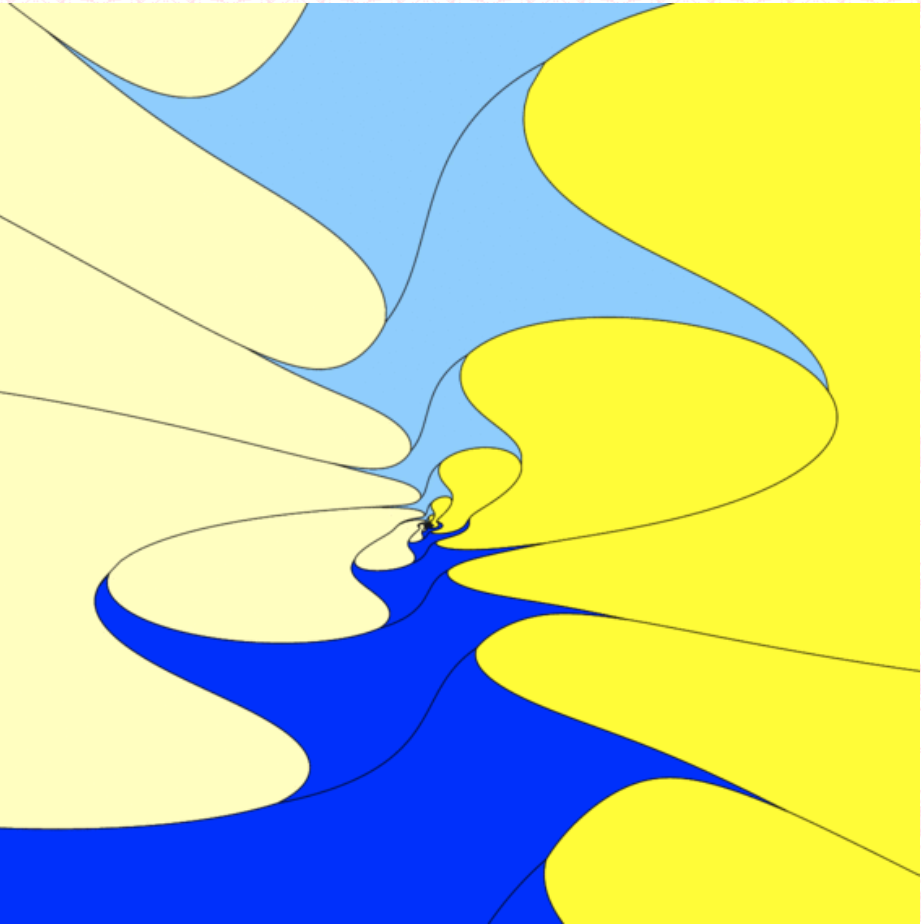
\includegraphics[scale=.15]{cplx_hyp.png} 
\end{center}


Another important class of discrete subgroups of $\mathrm{SU}(2,1)$ (or more
generally $\mathrm{SU}(n,1)$, 
or even more general Lie groups) is given by
holonomy groups of suitable geometric structures on moduli spaces 
In particular,
there is an important family of groups,
studied by Deligne-Mostow \cite{delignemostow}   and Thurston \cite{thurstonshapes},
which arise from
the moduli spaces of flat metrics on the sphere with fixed cone angle singularities.
This family is of special interest 
since it contains many of the 
known non-arithmetic lattices of $\mathrm{SU}(n,1)$.
Some parts of the  Deligne-Mostow-Thurston construction 
were extended by 
Veech \cite{veech}  to cover flat metrics on surfaces of positive genus.
Recently Ghazouani and Pirio \cite{ghazouanipirio}
have  pushed Veech's work a little further by 
but
the situation is still far from being completely understood -- for example it is not known which
holonomy groups are discrete, and if discrete, which are arithmetic.




\section{Objectives}
We now describe the main research challenges that we intend to tackle. 


\subsection{Combinatorial length and rigidity}
 Calculate the length
spectrum of a combinatorial surface, that is a graph which is
cellularly embedded in a surface.  For such a graph one associates a
length to each homotopy class of loops which is just the minimal
number of edges traversed by a circuit in the graph representing
it. The combinatorial length spectrum is the collection of all these
lengths. One can study the inverse spectral problem: to what extent
does this spectrum determine the surface? Exploring the connection of the length spectrum with graph Laplacian spectrum could be a promising angle of attack. Another intriguing question relates to the action of the mapping class group on this combinatorial length spectrum. Indeed, an automorphism of the
 surface permutes the homotopy class of curves, hence the length spectrum. Does the discrete nature of the graph metric induce specific properties of this action? In other words, can we learn the graph structure from this action?

\subsection{Algorithmic study of lengths}

Lazarus and Damiand have
added a package to the C++ library  CGAL which tests if two curves are
in the same free homotopy class. The algorithm test has linear
complexity: in about 30 seconds one can test two paths of
combinatorial length of 30 million on a surface of genus
100. The next step is to implement a test to see if a path
is homotopic to a simple loop. There is already an algorithm, of
“quasi”-linear complexity~\cite{dl-cginc-19}, which just needs to be implemented. With
this one can count the number of simple curves of length less than a given threshold 
and hopefully check the numerical values of certain important constants which
appear in the work of Mirzakhani.


\subsection{Curve complex}

Curver is a program for
performing calculations in the curve complex which implements the
Bell–Webb algorithm to determine the Nielsen–Thurston type of a
mapping class~\cite{b-c-17,b-esmt-19}. The algorithm runs in polynomial time but the constants
involved currently make this implementation impractical. There is a
sister program called Flipper\footnote{\url{https://markcbell.github.io/build/html/software.html}}which does calculations for surfaces
with boundary. There seems to be room to improve this situation and
implement this situation. Namely, finding a way of making the
algorithm practical by solving the problem of large constants and
extending the work to cover closed surfaces without boundary~\cite{mm-sosr-19}.

\subsection{General geometric structures}

Here we have two very concrete goals

\subsubsection{CR SnapPy}
As mentionned above would like to applying the  techniques developed 
by Schwartz, Deraux, Falbel, Parker, Will, in a
more systematic fashion so as to understand
which 3-manifolds admit a spherical CR structure.
Obviously since Week's SnapPea software 
has proved so useful in understanding 
hyperbolic structures on 3-manifolds
it would useful to have a similar tool
to explore CR structure.
So we hope to develop a spherical CR version of SnapPy,
which would allow the user to study, 
given a fundamental domain 
in complex hyperbolic space  for a
give discrete subgroup of $\mathrm{SU}(2,1)$, properties of the  manifold at infinity.


\subsubsection{Cellulations of moduli space}

To better understand the variations 
on the Deligne-Mostow-Thurston construction
of  Veech and Ghazouani-Pirio
it is important to understand the geometry
of tha associated moduli space.
We expect that a concrete understanding of their construction in terms of triangulations (or more general cell-decompositions) should given
insight into these open questions. 
If this produces complex hyperbolic
(or more general geometric) structures on some well-chosen moduli spaces, we expect that combinatorial methods will be crucial to understand the fine topological/geometric/dynamical structure of these
moduli spaces.

There are  natural cellulations of 
the moduli space hyperbolic (complex)  structures.
There are various constructions for these
due to amongst others Penner, Epstein-Penner,  Kontsevich.
Underlying these constructions 
are the lengths of certain curves on the surfaces
and embedded trivalent graphs.
The tri valent graph is dual to 
"the best possible" triangulation of the surface
in the Epstein-Penner construction
and this triangulation is obtained 
via the calculation of a convex hull
(which is computationally very cheap).
One hopes that interaction between team members
could lead to an extension of these constructions
to the space of flat moduli space 
and developping a computationally efficient
implementation.
 


\subsection{Harmonic maps}

A very important tool in the study of Teichm\" {u}ller space, namely the
space of deformation of Riemann surface structures, is represented by
harmonic maps \cite{wolf}. Harmony is  software developed in C++ by
Loustau and Gaster~\cite{glm-cdehm-18}, which computes harmonic maps between two
hyperbolic surfaces, described in terms of their Fenchel-Nielsen
coordinates, by means of a discrete heat flow method. In other words,
a hyperbolic surface is 
approximated by a finite graph 
which encodes its geometry, 
then one searches a discrete harmonic 
map by a  recursive procedure 
stopping when  a prescribed tolerance is reached. 
Very interesting developments would be
constituted by developing programs to compute harmonic maps with
target a metric tree, or a quasi-Fuchsian three-manifold, or to
compute minimal Lagrangian maps between closed hyperbolic surfaces \cite{BS}.


\section{Méthodologie envisagée}
%\textbf{mettant en avant la complémentarité des membres de l'équipe
%    (non nécessairement limitée au porteur)\\
%    dégageant les points durs qui feront l’objet d’un travail de thèse et/ou de post-doctorat
%}

Grenoble  has 
a very strong tradition both 
as a center for in low dimensional topology 
as well as for discrete mathematics and computer science
(including graph theory and some aspects of algorithms). 
We believe that the group of researchers from the Institut Fourier and G-SCOP 
involved
in this project posess a blend of complementary skills 
perfectly adapted
to working together on the objectives above.
On the one hand the G-SCOP team \emph{Optimisation Combinatoire} is certainly one of the leading groups in graph theory with an emphasis on topological aspects of graphs on surfaces~\cite{es-wqpp-18}. On the other the topology team at the Institut Fourier is a leading group in low dimensional topology 
especially the theory of surfaces 
with its many facets 
- dynamical, variational and spectral,
 interactions with classical and quantuum algebra.
 
More precisely:
\begin{itemize}
\item Martin Deraux is an expert in complex hyperbolic spaces. He has created programs in JAVA to determine 
\textit{fundamental domains} for groups acting on these spaces. This is a very delicate task and he must certify all his calculations so that they can be used in rigorously proving theorems.
\item Greg McShane has worked extensively on moduli of surfaces and the action of the mapping class group. He has discovered surprising relations between the moduli which can be used to explore the size and shape of the moduli space that is the space of all complex structures on a surface of fixed type.
\item Anne Parreau works on representations of the fundamental group of a surface into Lie groups. 
In her work there are functions which appear which generalise the lengths of curves on a surface.
\item Francis Lazarus is interested in the combinatorics of surfaces.

\end{itemize}

\vspace{.25in}



One of the things that makes
our proposal particularly relevant
at this time is that
the theme of the  Master of
Mathematics (M2R) for 2020-21
will be  geometric group theory, 
including its combinatorial aspects with applications to topology. 
In particular, Martin Deraud, Anne Parreau and Francis Lazarus will both be giving courses as part of  this Master. 
So accepting our proposal 
would be  an excellent opportunity 
to reinforce
what is at the moment a tentative synergy 
between team members in
quite distinct laboratories and
academic programs. 
The possibility to recrute 
students from these Masters courses
by offering fundings 
would be undoubtedly 
be good for the attractivity
of Grenoble as a place to study
both in the short and long term. 

Each of the challenges  in the above scientific description of the project
could certainly yield 
at least one subject for a PhD
in the context of this project.
Students would not only have the chance
to work with members of our team 
but would have interactions with
the  many seminar speakers 
in the geometry and topology seminars 
at the Institut Fourier
and the possibility of short visits
to other teams with whom the team members
have scientific collaborations
(ICJ Lyon, IMJ Paris, University of Luxembourg).




\section{Résultats attendus}
%\textbf{    les retombées scientifiques, techniques, logicielles,
%le potentiel de valorisation et/ou de pérennisation 
%}

The first challenge concerning the length spectrum of a combinatorial surface sits at the interface of graph theory and surface topology. Progress on this should provide a new point of view that fits perfectly in the structural approach of Robertson and Seymour. We are quite confident when we say  that there are few research groups with the same level of competence  in this domain.

The other challenges are related to implementations and experimental mathematics, 
which are again strengths of the 
mathematical/computer science community Grenoble. 
It is our intention to develop and distribute open source softwares and packages.

\section{Principales étapes envisagées}


\section{ Request budget and scientific justification}

We plan to hire one PhD students and one post-doctoral student. 
Both the PhD student
and the postdoctoral student
will be supervised jointly 
by members of the IF and the G-SCOP.
Ideally the PhD student would
come from the M2R at the IF 
in the academic year 2020-21.
Depending on the background of the student, the PhD thesis will focus on the
questions raised in sections ??.
The post-doctoral student is expected to have skills in both
theoretical mathematics 
and algorithms
to be involved in the research direction raised in section (??).

In addition to this, we plan to organize a workshop gathering all members of the
team and which could be entitled ”???” and several meetings
or one-day workshops with related ANR projects (???).
We also intend to organize 
a bimonthly all day meeting 
at which all members would participate
to reinforce the cohesion of the TOFU team
and facilitate the exchange of ideas.

A joint meeting of the SMF and AMS
will take place in June 2021
and we would like to organise a
special session.
This would be the perfect occasion to establish new contacts and identify promising questions where
geometry and computer science may fruitfully interact. In the same time it would dramatically
increase the visibility of our initiative and be an efficient way to attract very good post-doctoral
students.

\vspace{.5in}
 
\begin{itemize}

\item Financement de thèse : \hfill 100.000 \EUR\\
{\footnotesize Le sujet portera sur ...}
\item Post-doc (1 an) \hfill 50.000 \EUR\\
{\footnotesize ...}
\item Gratifications de stage : \hfill 6.000 \EUR\\
{\footnotesize correspondant à 3 stages M2 de 5 mois.}
\item Invitations de chercheurs extérieurs : \hfill 6.000 \EUR\\
{\footnotesize ...
}
\item Missions : \hfill 20.000 \EUR\\
{\footnotesize (1200\EUR par personne et par an)}
\item Matériel : \hfill 4.000 \EUR
\item Fonctionnement : \hfill 4.000 \EUR
\item Congrès-colloques :  \hfill 10.000 \EUR
\item TOTAL demandé : \hfill 200.000 \EUR
\end{itemize}


  \bibliographystyle{plain}

\bibliography{bibTofu}  

\end{document}